  \def\firstcircle{(0,0) circle (2cm)}
  \def\secondcircle{(2.3,1.8) circle (1.5cm)}
  \def\thirdcircle{(0,0) circle (1.5cm)}
  \colorlet{circle edge}{blue!50}
  \colorlet{circle area}{blue!20}
  \tikzset{filled/.style={fill=circle area, draw=circle edge, thick},
    outline/.style={draw=circle edge, thick}}
  \tikzstyle{important line}=[very thick]
  \centering
  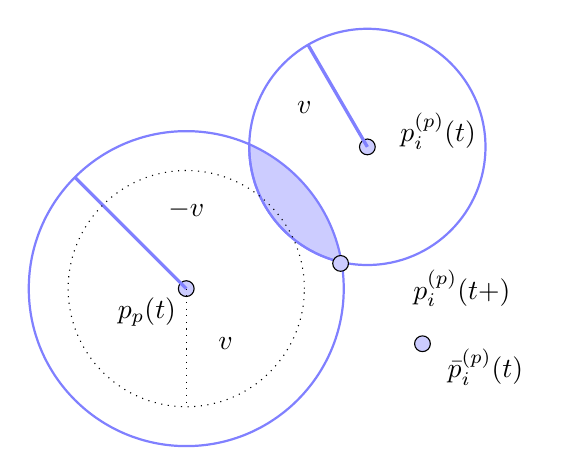
\begin{tikzpicture}
    \begin{scope}
        \clip \firstcircle;
        \fill[filled] \secondcircle;
    \end{scope}
    \draw[outline] \firstcircle node {$ $};
    \draw[fill=circle area] (0,0) circle (0.1cm); 
    \node at (-0.5,-0.3) {$p_p(t)$};
    \draw[style=important line, circle edge](90:1cm) -- node[black]{$\range- v\dt$}+(0,0);
   \draw[style=important line, circle edge](0,0) -- (135:2cm);
    \draw[outline] \secondcircle node {$ $};

    \draw[fill=circle area] (2.3,1.8) circle (0.1cm); 
    \node at (3.2, 2) {$p_i^{(p)}(t)$};

   \draw[style=important line, circle edge](2.3, 1.8) -- (1.55,3.09);
   \node at (1.5, 2.3) {$v\dt$};

    \draw[fill=circle area] (3, -0.7) circle (0.1cm); 
    \node at (3.8,-1) {$\bar{p}_i^{(p)}(t)$};
    \draw[dotted] \thirdcircle node{$ $};

   \draw[dotted](0, 0) -- (0,-1.5);
   \node at (0.5, -0.7) {$v\dt$};

  \draw[fill=circle area] (1.96, 0.32) circle (0.1cm); 
    \node at (3.5,0) {${p}_i^{(p)}(t+\dt)$};
  \end{tikzpicture}
  \caption{The real destination for the descendant robot $r_i$ to maintain connected with its parent $r_p$ during time $t+\dt$.}